\documentclass[10pt,letterpaper]{article}

\usepackage[margin=0.78in]{geometry}
\usepackage[T1]{fontenc}
\usepackage[utf8]{inputenc}
\usepackage{lmodern}
\usepackage{microtype}
\usepackage{booktabs}
\usepackage{array}
\usepackage{longtable}
\usepackage{xcolor}
\usepackage{hyperref}
\usepackage{tikz}
\usepackage{graphicx}
\usepackage{float}
\usetikzlibrary{arrows.meta,positioning,shapes.geometric,fit}

\hypersetup{
  colorlinks=true,
  linkcolor=black,
  urlcolor=blue
}

\definecolor{softgray}{HTML}{F2F4F7}
\definecolor{softblue}{HTML}{EAF2F8}
\definecolor{softorange}{HTML}{FFF0E6}
\definecolor{softgreen}{HTML}{EAF7EA}
\definecolor{lineblue}{HTML}{1F4E79}
\definecolor{lineorange}{HTML}{C55A11}
\definecolor{linegreen}{HTML}{2E7D32}

\title{\textbf{Stage 1 IBR Version Report: IEEE 39 \texttt{mix60} Case}}
\author{Conversion documentation for \texttt{data/processed/mix60/mix60.xlsx}}
\date{Generated from \texttt{conversion\_protocol.yaml} and ANDES workbook contents}

\begin{document}
\maketitle

\begin{abstract}
This document describes the generated IBR version of the IEEE 39 dynamic case,
profile \texttt{mix60}. It explains which generator buses were changed, which
dynamic records were removed, which ANDES IBR records were added, and which
variables are copied from the original static generator data versus assigned
from the configured parameter profiles. The report is about the case
construction itself, not about the later time-domain comparison.
\end{abstract}

\section{Case Identity}

\begin{center}
\begin{tabular}{ll}
\toprule
Item & Value \\
\midrule
Protocol & \texttt{ieee39\_ibr\_conversion\_protocol} \\
Active profile & \texttt{mix60} \\
Base workbook & \texttt{data/raw/ieee39\_full.xlsx} \\
Generated IBR workbook & \texttt{data/processed/mix60/mix60.xlsx} \\
Build manifest & \texttt{outputs/stage1\_build\_ibr\_case/mix60/manifest.json} \\
ANDES version in manifest & \texttt{2.0.0} \\
Power-flow policy & preserve the original static \texttt{PV}/\texttt{Slack} dispatch \\
\bottomrule
\end{tabular}
\end{center}

The conversion changes the dynamic resource representation, not the solved
network topology. Static network sheets such as \texttt{Bus}, \texttt{PQ},
\texttt{PV}, \texttt{Slack}, \texttt{Shunt}, \texttt{Line}, and \texttt{Area}
are preserved. The static generator injections remain in \texttt{PV} and
\texttt{Slack}; the replacement is made in the dynamic model sheets.

\section{Profile Logic}

The protocol declares buses 31--38 as eligible conversion sites and keeps buses
30, 31, 32, and 39 synchronous in \texttt{mix60}. Bus 39 is retained because it
represents the external interconnection/equivalent.

\begin{center}
\begin{tabular}{lll}
\toprule
Resource group & Generator indices & Bus indices \\
\midrule
Kept synchronous & 1, 2, 3, 10 & 30, 31, 32, 39 \\
Converted to GFL & 5, 7, 9 & 34, 36, 38 \\
Converted to GFM & 4, 6, 8 & 33, 35, 37 \\
\bottomrule
\end{tabular}
\end{center}

\section{Conversion Matrix}

\begin{center}
\resizebox{\linewidth}{!}{%
\begin{tabular}{clllll}
\toprule
Generator & Bus & Static record & Base dynamic records removed & New IBR records & Role \\
\midrule
1 & 30 & \texttt{PV 1} & none & none & synchronous retained \\
2 & 31 & \texttt{PV 2} & none & none & synchronous retained \\
3 & 32 & \texttt{PV 3} & none & none & synchronous retained \\
4 & 33 & \texttt{PV 4} &
\texttt{GENROU\_4, TGOV1\_4, IEEEX1\_4, IEEEST\_4} &
\texttt{REGF1\_G4} & GFM \\
5 & 34 & \texttt{PV 5} &
\texttt{GENROU\_5, TGOV1\_5, IEEEX1\_5, IEEEST\_5} &
\texttt{PLL1\_G5, REGCP1\_G5, REECA1\_G5, REPCA1\_G5} & GFL \\
6 & 35 & \texttt{PV 6} &
\texttt{GENROU\_6, TGOV1\_6, IEEEX1\_6, IEEEST\_6} &
\texttt{REGF1\_G6} & GFM \\
7 & 36 & \texttt{PV 7} &
\texttt{GENROU\_7, TGOV1\_7, IEEEX1\_7, IEEEST\_7} &
\texttt{PLL1\_G7, REGCP1\_G7, REECA1\_G7, REPCA1\_G7} & GFL \\
8 & 37 & \texttt{PV 8} &
\texttt{GENROU\_8, TGOV1\_8, IEEEX1\_8, IEEEST\_8} &
\texttt{REGF1\_G8} & GFM \\
9 & 38 & \texttt{PV 9} &
\texttt{GENROU\_9, TGOV1\_9, IEEEX1\_9, IEEEST\_9} &
\texttt{PLL1\_G9, REGCP1\_G9, REECA1\_G9, REPCA1\_G9} & GFL \\
10 & 39 & \texttt{Slack 10} & none & none & synchronous external equivalent \\
\bottomrule
\end{tabular}
}
\end{center}

\section{ANDES Sheet-Level Delta}

\begin{center}
\begin{tabular}{lccp{6.2cm}}
\toprule
Sheet & Base rows & \texttt{mix60} rows & Meaning \\
\midrule
\texttt{GENROU} & 10 & 4 & Synchronous machine dynamics retained only for generators 1, 2, 3, 10. \\
\texttt{TGOV1N} & 10 & 4 & Governor records retained only for synchronous machines. \\
\texttt{IEEEX1} & 10 & 4 & Exciter records retained only for synchronous machines. \\
\texttt{IEEEST} & 10 & 4 & Stabilizer records retained only for synchronous machines. \\
\texttt{PLL1} & 0 & 3 & PLLs added for the GFL chain at buses 34, 36, 38. \\
\texttt{REGCP1} & 0 & 3 & Converter interface model for GFL resources. \\
\texttt{REECA1} & 0 & 3 & Electrical controller for GFL resources. \\
\texttt{REPCA1} & 0 & 3 & Plant controller for GFL resources. \\
\texttt{REGF1} & 0 & 3 & Grid-forming inverter model at buses 33, 35, 37. \\
\texttt{PV} & 9 & 9 & Static active/reactive dispatch preserved. \\
\texttt{Slack} & 1 & 1 & External/slack generator preserved. \\
\bottomrule
\end{tabular}
\end{center}

\section{Conversion Diagram}

\begin{figure}[H]
\centering
\resizebox{\linewidth}{!}{%
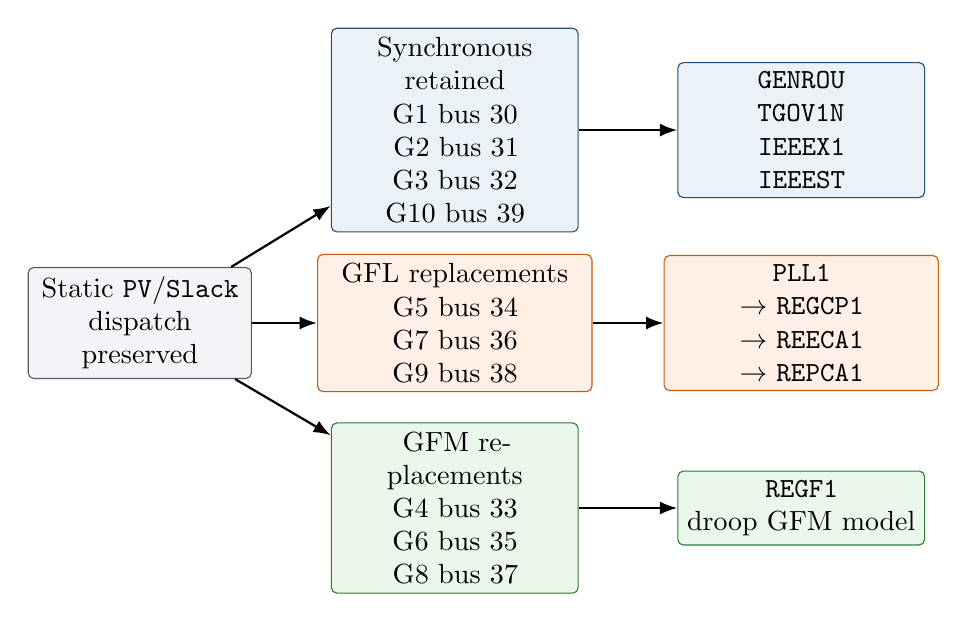
\begin{tikzpicture}[
  bus/.style={
    rectangle, rounded corners=2pt, draw=black!65, fill=softgray,
    align=center, minimum height=0.8cm, text width=2.6cm
  },
  sg/.style={
    rectangle, rounded corners=2pt, draw=lineblue, fill=softblue,
    align=center, minimum height=0.8cm, text width=2.9cm
  },
  gfl/.style={
    rectangle, rounded corners=2pt, draw=lineorange, fill=softorange,
    align=center, minimum height=0.8cm, text width=3.25cm
  },
  gfm/.style={
    rectangle, rounded corners=2pt, draw=linegreen, fill=softgreen,
    align=center, minimum height=0.8cm, text width=2.9cm
  },
  arrow/.style={-{Latex[length=2.2mm]}, thick}
]
\node[bus] (pv) at (0,0) {Static \texttt{PV}/\texttt{Slack}\\dispatch preserved};

\node[sg] (sg) at (4.0,2.45) {
Synchronous retained\\
G1 bus 30\\G2 bus 31\\G3 bus 32\\G10 bus 39};

\node[gfl] (gfl) at (4.0,0) {
GFL replacements\\
G5 bus 34\\G7 bus 36\\G9 bus 38};

\node[gfm] (gfm) at (4.0,-2.35) {
GFM replacements\\
G4 bus 33\\G6 bus 35\\G8 bus 37};

\node[sg] (sgchain) at (8.4,2.45) {
\texttt{GENROU}\\
\texttt{TGOV1N}\\
\texttt{IEEEX1}\\
\texttt{IEEEST}};

\node[gfl] (gflchain) at (8.4,0) {
\texttt{PLL1}\\
\(\rightarrow\) \texttt{REGCP1}\\
\(\rightarrow\) \texttt{REECA1}\\
\(\rightarrow\) \texttt{REPCA1}};

\node[gfm] (gfmchain) at (8.4,-2.35) {
\texttt{REGF1}\\
droop GFM model};

\draw[arrow] (pv) -- (sg);
\draw[arrow] (pv) -- (gfl);
\draw[arrow] (pv) -- (gfm);
\draw[arrow] (sg) -- (sgchain);
\draw[arrow] (gfl) -- (gflchain);
\draw[arrow] (gfm) -- (gfmchain);
\end{tikzpicture}
}
\caption{Dynamic model architecture of the \texttt{mix60} IBR workbook. Static
dispatch remains in the \texttt{PV}/\texttt{Slack} sheets; dynamic records are
replaced only for the selected generator sites.}
\end{figure}

\section{Variable Provenance}

The conversion uses two sources of variables: static generator values from the
original \texttt{PV}/\texttt{Slack} rows, and controller parameters declared in
\texttt{configs/cases/conversion\_protocol.yaml}. The table below summarizes
the main provenance rules.

\begin{longtable}{p{2.7cm}p{4.5cm}p{6.1cm}}
\toprule
New sheet/model & Variables copied from original case & Variables assigned by profile/defaults \\
\midrule
\endhead
\texttt{PLL1} &
\texttt{bus} from the converted generator bus. &
\texttt{Kp=1}, \texttt{Ki=0.2}, \texttt{Tf=0.05}, \texttt{Tp=0.05}, \texttt{fn=60}. \\
\texttt{REGCP1} &
\texttt{bus}, \texttt{gen}, and \texttt{Sn}; \texttt{pll} links to the new \texttt{PLL1} record. &
\texttt{Tg=0.1}, \texttt{Rrpwr=10}, \texttt{Brkpt=1}, \texttt{Zerox=0.5}, \texttt{Volim=1.2}, \texttt{Khv=0.7}, current limits and gains from \texttt{published\_gfl\_baseline}. \\
\texttt{REECA1} &
\texttt{reg} links to the new \texttt{REGCP1}; \texttt{Vref0} and \texttt{Vref1} use original \texttt{v0}. &
Voltage ride-through, current limit, PI gains, and broad limits such as \texttt{Imax=10}, \texttt{QMax=999}, \texttt{PMAX=999}. \\
\texttt{REPCA1} &
\texttt{ree} links to the new \texttt{REECA1}; \texttt{busf} links to the matching \texttt{BusFreq} record. &
Plant control flags and gains: \texttt{VCFlag=1}, \texttt{RefFlag=1}, \texttt{Kp=1}, \texttt{Ki=0.1}, \texttt{Ddn=10}, \texttt{Dup=10}. \\
\texttt{REGF1} &
\texttt{bus}, \texttt{gen}, \texttt{Sn}; \texttt{rf} from \texttt{PV.ra}; \texttt{xf} from \texttt{PV.xs} unless overridden; \texttt{Pmax/Pmin/Qmax/Qmin} from static generator limits. &
GFM control parameters: \texttt{wdrp=0.033}, \texttt{Qdrp=0.045}, \texttt{Tr=0.005}, \texttt{Te=0.005}, current/voltage PI gains, and \texttt{Tpm=0.025}. \\
\bottomrule
\end{longtable}

\section{Added IBR Records}

\subsection{Grid-Following Chain}

\begin{center}
\begin{tabular}{llllll}
\toprule
Gen & Bus & PLL & Converter & Electrical control & Plant control \\
\midrule
5 & 34 & \texttt{PLL1\_G5} & \texttt{REGCP1\_G5} & \texttt{REECA1\_G5} & \texttt{REPCA1\_G5} \\
7 & 36 & \texttt{PLL1\_G7} & \texttt{REGCP1\_G7} & \texttt{REECA1\_G7} & \texttt{REPCA1\_G7} \\
9 & 38 & \texttt{PLL1\_G9} & \texttt{REGCP1\_G9} & \texttt{REECA1\_G9} & \texttt{REPCA1\_G9} \\
\bottomrule
\end{tabular}
\end{center}

These are configured as GFL because the converter uses \texttt{REGCP1} with a
PLL and a \texttt{REECA1}/\texttt{REPCA1} control chain. The plant controller
uses the corresponding \texttt{BusFreq} record for the generator bus.

\subsection{Grid-Forming Records}

\begin{center}
\begin{tabular}{llllll}
\toprule
Gen & Bus & New model & \texttt{Sn} & \texttt{Pmax} & \texttt{Qmax} \\
\midrule
4 & 33 & \texttt{REGF1\_G4} & 1174.8 & 6.82 & 5.48208 \\
6 & 35 & \texttt{REGF1\_G6} & 1085.7 & 6.97 & 5.93788 \\
8 & 37 & \texttt{REGF1\_G8} & 970.2 & 5.64 & 4.43468 \\
\bottomrule
\end{tabular}
\end{center}

These are configured as GFM because the dynamic replacement is \texttt{REGF1},
using droop parameters \texttt{wdrp=0.033} and \texttt{Qdrp=0.045}, with active
and reactive limits copied from the original static generator rows.

\section{Removed Dynamic Records}

For the converted generators 4--9, the synchronous machine and its associated
governor, exciter, and stabilizer records are removed:

\begin{center}
\resizebox{\linewidth}{!}{%
\begin{tabular}{llll}
\toprule
\texttt{GENROU} removed & \texttt{TGOV1N} removed & \texttt{IEEEX1} removed & \texttt{IEEEST} removed \\
\midrule
\texttt{GENROU\_4} & \texttt{TGOV1\_4} & \texttt{IEEEX1\_4} & \texttt{IEEEST\_4} \\
\texttt{GENROU\_5} & \texttt{TGOV1\_5} & \texttt{IEEEX1\_5} & \texttt{IEEEST\_5} \\
\texttt{GENROU\_6} & \texttt{TGOV1\_6} & \texttt{IEEEX1\_6} & \texttt{IEEEST\_6} \\
\texttt{GENROU\_7} & \texttt{TGOV1\_7} & \texttt{IEEEX1\_7} & \texttt{IEEEST\_7} \\
\texttt{GENROU\_8} & \texttt{TGOV1\_8} & \texttt{IEEEX1\_8} & \texttt{IEEEST\_8} \\
\texttt{GENROU\_9} & \texttt{TGOV1\_9} & \texttt{IEEEX1\_9} & \texttt{IEEEST\_9} \\
\bottomrule
\end{tabular}
}
\end{center}

\section{What Did Not Change}

\begin{itemize}
  \item The bus and line network topology is not rewritten by this conversion.
  \item \texttt{PV} and \texttt{Slack} rows are preserved to keep the same
  static dispatch and voltage setpoints.
  \item \texttt{PQ} load rows are not changed by the IBR conversion.
  \item \texttt{BusFreq} rows are preserved for all generator buses and are
  linked where needed by \texttt{REPCA1}.
  \item The disabled original \texttt{Toggler\_1} for \texttt{GENROU\_1} remains
  disabled in the generated workbook.
\end{itemize}

\section{Important Engineering Notes}

\begin{enumerate}
  \item The conversion is a controlled research transformation, not a canonical
  official IEEE 39 IBR benchmark.
  \item The static power flow is intentionally preserved. Therefore, the IBR
  version should start from the same solved dispatch as the base case.
  \item The GFL parameter set uses broad controller limits, for example
  \texttt{Imax=10} and wide active/reactive limits in \texttt{REECA1} and
  \texttt{REPCA1}. These are useful for an initial reproducible build, but they
  should be tightened or justified before making strong physical claims.
  \item The GFM \texttt{REGF1} records inherit physical limits from the original
  static generator rows, while their droop and inner-loop gains come from the
  configured profile.
  \item The generated case must still be validated with dynamic gates. A case
  can be structurally correct and still show questionable voltage or stability
  behavior under specific contingencies.
\end{enumerate}

\section{Reproduction Commands}

The IBR workbook can be rebuilt with:

\begin{verbatim}
$env:SYMPY_GROUND_TYPES='python'
$env:PYTHONPATH='src'
python -m spectral_ibr.interface.cli gate run stage1-build-ibr-case --profile mix60
\end{verbatim}

The dynamic comparison can then be run separately with:

\begin{verbatim}
$env:SYMPY_GROUND_TYPES='python'
$env:PYTHONPATH='src'
python -m spectral_ibr.interface.cli gate run stage1-td-compare --profile mix60
\end{verbatim}

\section{Summary}

The \texttt{mix60} workbook is the IBR version of the IEEE 39 dynamic case in
which six generator dynamic models are replaced while preserving the static
dispatch. Buses 34, 36, and 38 become GFL sites using the
\texttt{PLL1 -> REGCP1 -> REECA1 -> REPCA1} chain. Buses 33, 35, and 37 become
GFM sites using \texttt{REGF1}. Buses 30, 31, 32, and 39 remain synchronous.
This is the structural change that creates the IBR case; subsequent plots and
TDS results are validation of this case, not the definition of the case itself.

\end{document}
